\documentclass[../../main.tex]{subfiles}

\begin{document}
\section{Lavoro, Energia e Momenti}
\[
    dW = dL = \vec{F} \cdot d\vec{s} \ \text{ lavoro infinitesimo compiuto da } \ \vec{F}
\]
\[
    F(x,y,z) \text{ lavoro compiuto dalla forza $F$ quando è andato da A a B lungo } \Gamma
\]
Dove $\Gamma$ è la curva che congiunge A e B.\\
Il lavoro è la somma di tutti i lavori infinitesimi:
\[
    W = \int_{A}^{B} \vec{F} \cdot d\vec{s} = \int_{A}^{B} F_T ds
\]
\[
    F_T = F \cos \theta
\]
Integrale di linea del lavoro di una forza lungo una curva $\Gamma$.
\[
    W_1 = \int_A^B \vec{F_1} \cdot d\vec{s} \quad W_2 = \int_A^B \vec{F_2} \cdot d\vec{s} \quad W_3 = \int_A^B \vec{F_3} \cdot d\vec{s} \implies \vec F = \vec F_1 + \vec F_2 + \vec F_3 \implies W = \int_{A}^{B} \vec{F} \cdot d\vec{s} = W_1 + W_2 + W_3
\]
\[
    [L] = \dfrac{kg\cdot m^2}{s^2}
\]
\subsection{Potenza}
\[
    P = \frac{dW}{dt} = \dfrac{d(\vec F \cdot \vec s)}{dt} = \vec F \dfrac{d\vec s}{dt} = \vec F \cdot \vec v
\]
\[
    [\text{Potenza}] = \dfrac{kg\cdot m^2}{s^3} = W
\]
\[
    P_m = \dfrac{L_{\text{totale}}}{\Delta t}
\]
\subsection{Teorema per il 18 - Th energia cinetica}
\[
    dW = \vec F\cdot d\vec s = F_T\cdot ds = ma_T ds = m\dfrac{dv}{dt}\cdot ds = m\cdot vdv
\]
\begin{mdframed}[outerlinecolor=red,outerlinewidth=1pt,linecolor=cccolor,roundcorner=10pt]
    \[
        W = \int_{v_A}^{v_B} m\cdot vdv = \dfrac{1}{2}mv_B^2 - \dfrac{1}{2}mv_A^2
    \]
\end{mdframed}
dove $\dfrac{1}{2} mv^2$ è l'energia cinetica e la differenza tra l'energia cinetica finale e quella iniziale si indica con $\Delta E_k$.

\subsection{Lavoro della forza peso}
\begin{figure}[H]
    \centering
    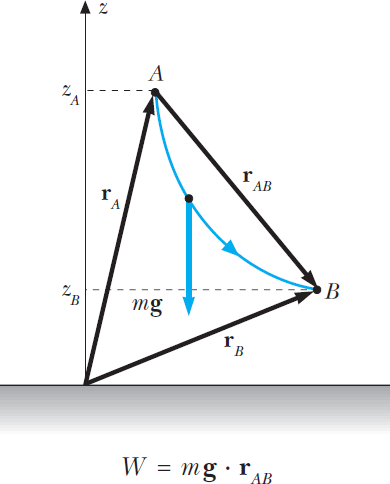
\includegraphics[width=0.3\textwidth]{Graphics-011.png}
\end{figure}
\[
    W = \int_{A}^{B} \vec F\cdot d\vec s = \vec F \int_{A}^{B} d\vec s = \vec F \cdot \vec r_{AB} = -m\vec g \cdot \vec r_{AB} = -mg(z_B - z_A) \implies -(mgz_B - mgz_A)
\]
La forza peso è una \textbf{forza conservativa}.
\subsection{Esempio 4.1}
Un punto di massa $m$ si trova alla base di un piano inclinato liscio; se la velocità iniziale vale $v_A$ ed è diretta come in Figura, calcolare qual è l’altezza rispetto alla base della posizione in cui il punto si ferma.\\
\begin{minipage}{0.3\textwidth}
    \centering
    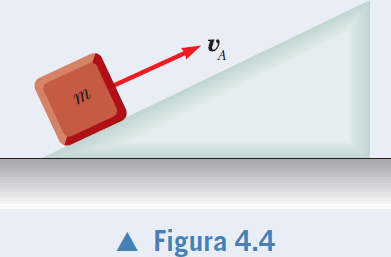
\includegraphics[width=1\textwidth]{Graphics-014.png}
\end{minipage}
\begin{minipage}{0.7\textwidth}
    \centering
    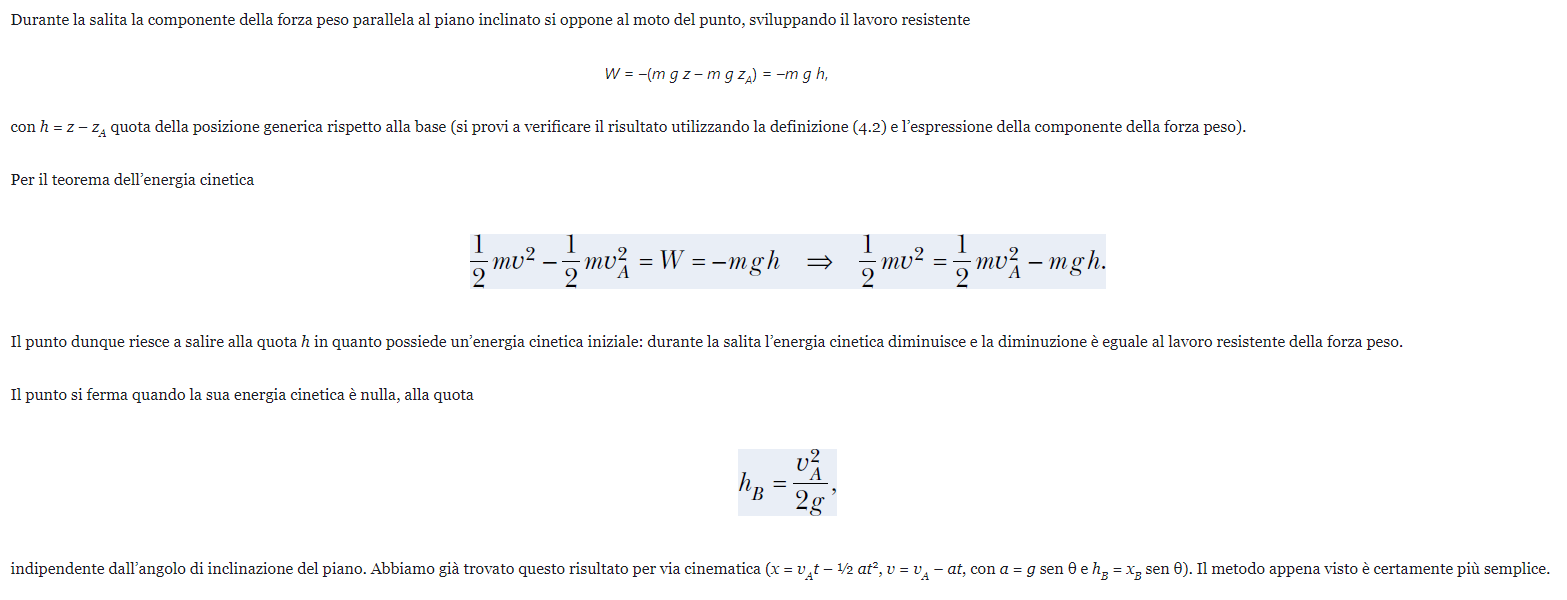
\includegraphics[width=1\textwidth]{4.1sol.png}
\end{minipage}
\subsection{Esempio 4.2}
Un punto materiale fissato a una molla di costante elastica k è in quiete nell’origine, Figura. Si applica al punto una forza $\vec F = F \vec u_x$, costante in modulo, direzione e verso, e il punto si muove lungo x. Calcolare la velocità del punto in funzione di x e la posizione in cui il punto si ferma.
\begin{minipage}
    {0.3\textwidth}
    \centering
    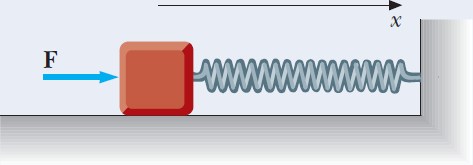
\includegraphics[width=1\textwidth]{Graphics-019.png}
\end{minipage}
\begin{minipage}{0.7\textwidth}
    \centering
    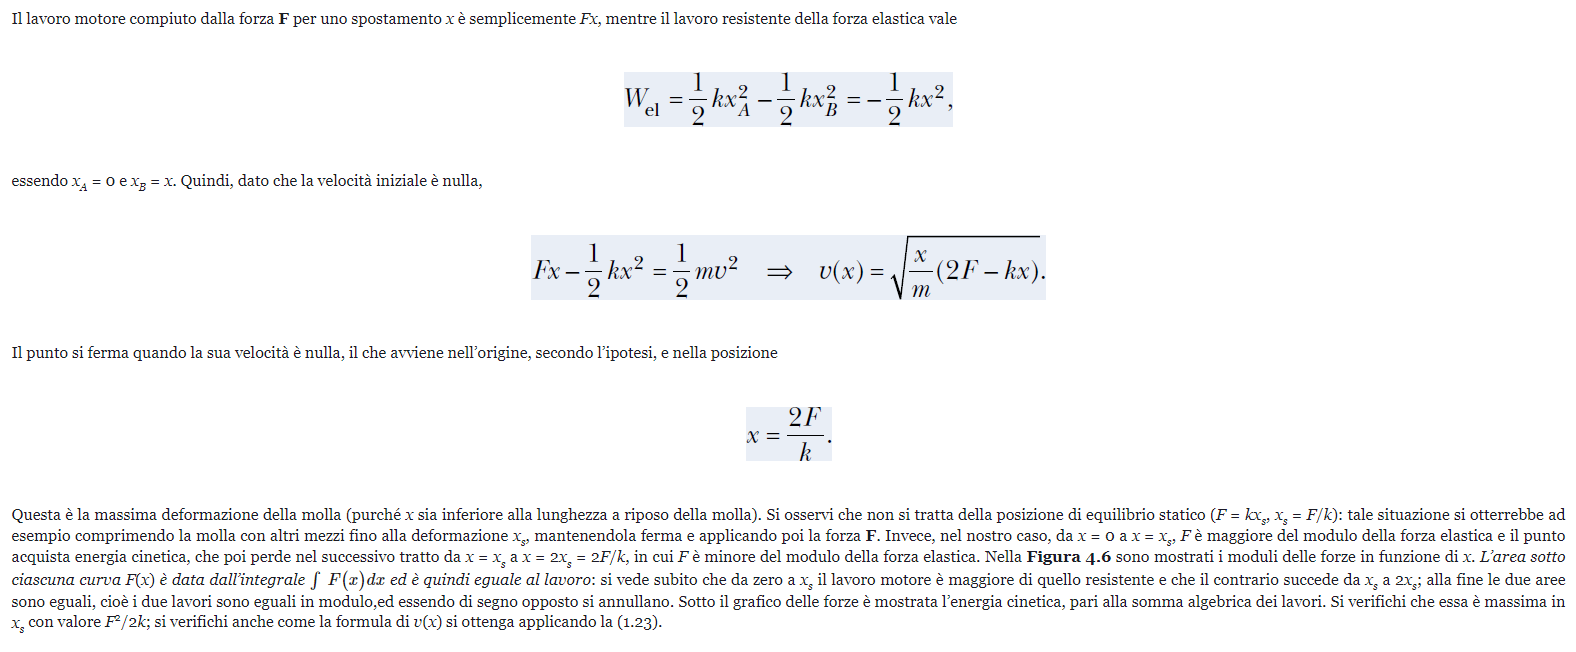
\includegraphics[width=1\textwidth]{4.2sol.png}
\end{minipage}

\end{document}